\documentclass{rapportECL2024}

\addbibresource{biblio.bib}
\newcommand{\var}[1]{\texttt{#1}}
\newcommand{\func}[1]{\small\texttt{#1}}
%--------------------------------------

\titre{Projet de programmation numérique}
\soustitre{Méthodes ensemblistes pour la modélisation}

\enseignant{Mathys \textsc{JAM}}

\eleves{Yifan \textsc{LI} \\
	Nicolas \textsc{DAIX-MOREUX} \\ 
	Brendan \textsc{FIXOT} \\
    Dorian \textsc{DRIVET}
    }
%--------------------------------------

\begin{document}

\fairepagedegarde
\fairetabledesmatieres

%--------------------------------------

\section{Arbre de régression}


Un arbre de régression est un modèle d'apprentissage supervisé conçu pour résoudre des problèmes où la variable cible est continue. Il fonctionne en partitionnant les données en sous-groupes de plus en plus homogènes, en fonction de seuils appliqués aux différentes caractéristiques des données. Chaque nœud interne de l'arbre correspond à une condition, tandis que chaque feuille représente une prédiction, généralement la moyenne des valeurs cibles des données associées à cette feuille.

L'objectif principal d'un arbre de régression est de prédire une valeur numérique avec précision en exploitant les relations entre les caractéristiques d'entrée et la variable cible. Par exemple, dans le cadre de ce projet, l'arbre sera utilisé pour prédire la performance d'un programme en fonction de divers paramètres qui ont été anonymisés ou bien la taille des matrices.

L'un des principaux avantages des arbres de régression est leur interprétabilité : leur structure hiérarchique permet de visualiser facilement les décisions prises par le modèle. De plus, ils peuvent capturer des relations non linéaires et des interactions complexes entre les caractéristiques, sans nécessiter un prétraitement approfondi des données. Ces qualités en font un bon outil pour analyser des données et fournir des prédictions précises, tout en restant compréhensible pour les utilisateurs.


\subsection{Construction de l'arbre}
\subsubsection{Introduction}
La construction d'un arbre de régression repose sur un processus récursif qui divise les données en sous-groupes homogènes en fonction des caractéristiques des données et d'une mesure de qualité de division. Dans ce projet, l'arbre est construit en utilisant des critères tels que la minimisation de la variance (Mean Squared Error, MSE) ou l'erreur absolue moyenne (Mean Absolute Error, MAE). Chaque nœud interne de l'arbre correspond à une condition de division, et chaque feuille représente une prédiction basée sur les données de son groupe.

L'algorithme développé dans ce projet inclut des étapes clés : la gestion des paramètres de profondeur maximale et de taille minimale des feuilles, la recherche du meilleur point de division, et l'arrêt conditionnel pour éviter le sur-apprentissage.

\subsubsection{Processus de divison des noeuds}
Le processus de construction de l'arbre commence par un appel à la méthode \func{train}, qui initialise l'arbre et appelle la fonction récursive \func{splitNode}. Cette dernière effectue les tâches suivantes :

Calcul de la qualité actuelle du nœud : La qualité du nœud est mesurée en utilisant l'erreur quadratique moyenne ou l'erreur absolue moyenne, calculé à partir des labels associés aux indices des données.

Conditions d'arrêt : La division d'un nœud s'arrête si l'une des conditions suivantes est remplie :
La profondeur maximale définie \var{MaxDepth} est atteinte.
Le nombre de données dans un nœud est inférieur à une taille minimale \var{MinLeafLarge}.
L'erreur actuelle est inférieure à un seuil prédéfini \var{MinError}.

Recherche du meilleur point de division : La méthode findBestSplit ou findBestSplitUsingMAE est utilisée pour identifier le meilleur attribut et le meilleur seuil qui minimisent l'erreur après la division.

Division des données : Les données sont séparées en deux sous-groupes (gauche et droite) en fonction du seuil identifié. Chaque sous-groupe est traité récursivement.

\subsection{Prétraitement des données}
Le prétraitement des données constitue une étape essentielle pour garantir la qualité et la fiabilité des données utilisées dans la construction de l'arbre de régression. Il permet d'éliminer les valeurs aberrantes, de structurer les données et de réduire les biais potentiels. Voici les principales étapes et les fonctions associées.


\subsubsection{Source de données}
L'ensemble de données utilisé dans ce projet contient les résultats d'un programme exécuté dans diverses configurations. Ce programme est un outil de benchmarking pour le noyau dgetrf (décomposition LU) de la bibliothèque LAPACK. Bien que le benchmark utilise des méta-répétitions, les résultats de mesure sont toujours bruyants d'environ $10\%$

\subsubsection{Structure et lecture des données}
Le prétraitement des données commence par la fonction \texttt{readCSV}, qui permet de charger les données brutes à partir d'un fichier CSV. Cette fonction lit le fichier ligne par ligne et analyse chaque ligne pour la convertir en une structure \texttt{DataRow}. Chaque enregistrement de données contient les informations clés suivantes :
\begin{itemize}
    \item \textbf{values} : les valeurs complètes de toutes les colonnes des données brutes.
    \item \textbf{matrix\_size\_x} et \textbf{matrix\_size\_y} : les dimensions de la matrice extraites du CSV.
    \item \textbf{performance} : les données de performance (la performance du programme sous différentes configurations).
\end{itemize}
Après avoir chargé et structuré les données, le programme utilise la fonction 
 \texttt{writeCSV} pour enregistrer les données nettoyées dans un nouveau fichier \texttt{CSV}. Cette fonction conserve l'en-tête du tableau d'origine et écrit les données valides vérifiées ligne par ligne, fournissant ainsi un format de données standardisé pour la formation ultérieure du modèle d'arbre de décision.
\subsubsection{Détection et nettoyage des valeurs aberrantes}
Selon la présence de dix pour cent de bruit (valeurs aberrantes) dans les résultats de mesure. Afin d'améliorer la précision et la robustesse du modèle, des méthodes de nettoyage globales et locales sont ajoutées au prétraitement des données. Un filtrage efficace des valeurs aberrantes dans l'ensemble de données est obtenu grâce à des techniques de \texttt{Z-score} et de regroupement.

\paragraph{1.Nettoyage basé sur le Z-score global}
La fonction \texttt{RemoveOutliers} utilise la méthode \texttt{Z-score} pour détecter et nettoyer les valeurs aberrantes globales. Sa mise en œuvre spécifique comprend les étapes suivantes :
\subparagraph{Calcul de la moyenne et de l'écart type}
Calculez la moyenne et l'écart type des données de performance pour mesurer la tendance centrale et la dispersion des données. La formule est la suivante :
\[
\text{mean} = \frac{1}{n} \sum_{i=1}^{n} x_i, \quad 
\text{stdDev} = \sqrt{\frac{1}{n} \sum_{i=1}^{n} (x_i - \text{mean})^2}
\]
\subparagraph{Détermination des valeurs aberrantes}
Calculez le score Z de chaque élément de données selon la formule suivante:
\[
Z = \frac{x - \text{mean}}{\text{stdDev}}
\]
Si le score Z d'une donnée dépasse le seuil prédéfini, il sera considéré comme une valeur aberrante et supprimé. Ce seuil représente la plage acceptable d'écart des données par rapport à la moyenne et correspond généralement à environ 95 $\%$ des données conservées.
\subparagraph{Filtrage des données}
Pour chaque élément de données, déterminez si son score Z se situe dans la plage définie. Seuls les enregistrements répondant aux critères sont conservés et le reste des données est supprimé.
\paragraph{2. Nettoyage partiel basé sur le binning} 
Dans le cas d'une distribution inégale des données (distribution gaussienne), un nettoyage global unique peut ne pas suffire à capturer les valeurs aberrantes locales. De plus, plusieurs cycles de nettoyage complet risquent de conduire à une suppression excessive des données, compromettant ainsi la préservation de leurs caractéristiques. Pour remédier à cela, une méthode de détection des valeurs aberrantes locales basée sur le regroupement (\textit{binning}) est introduite. Les données sont regroupées en fonction de la taille de la matrice (\texttt{matrix\_size\_x} et \texttt{matrix\_size\_y}). La mise en œuvre spécifique de cette méthode comprend les étapes suivantes :
\subparagraph{Binning}
Utilisez la fonction \texttt{equalFrequencyBinning} pour effectuer un regroupement à fréquence égale sur les données. Cette méthode trie les valeurs de \texttt{matrix\_size\_x} et \texttt{matrix\_size\_y} par ordre croissant et divise les données en un nombre fixe de groupes, chaque groupe contenant approximativement le même nombre de points de données. La formule de regroupement est la suivante :
\[
\text{binIndex}_i = \min\left(\left\lfloor \frac{i}{\text{binSize}} \right\rfloor, \text{numBins} - 1\right)
\]
Parmi eux, \texttt{binSize} est le nombre de points de données dans chaque bac et \texttt{numBins} est le nombre total de bacs.
\subparagraph{Détection des valeurs aberrantes locales}
Pour chaque groupe, extrayez ses données de performance internes (performance), calculez respectivement la moyenne et l'écart type et détectez les valeurs aberrantes en fonction du score Z. La formule est la même que pour le nettoyage global, mais la portée de détection est limitée aux données du bac actuel. Grâce à ce traitement local, les valeurs aberrantes régionales dans la distribution des données peuvent être capturées.
\paragraph{3.Analyse des performances du prétraitement des données}
Grâce au prétraitement des données, comme le montre la figure ci-dessous, nous pouvons nettoyer et ajuster de manière significative les valeurs aberrantes mondiales et locales. Le modèle de prétraitement des données a bien fonctionné.
\begin{figure}[h!] 
    \centering
    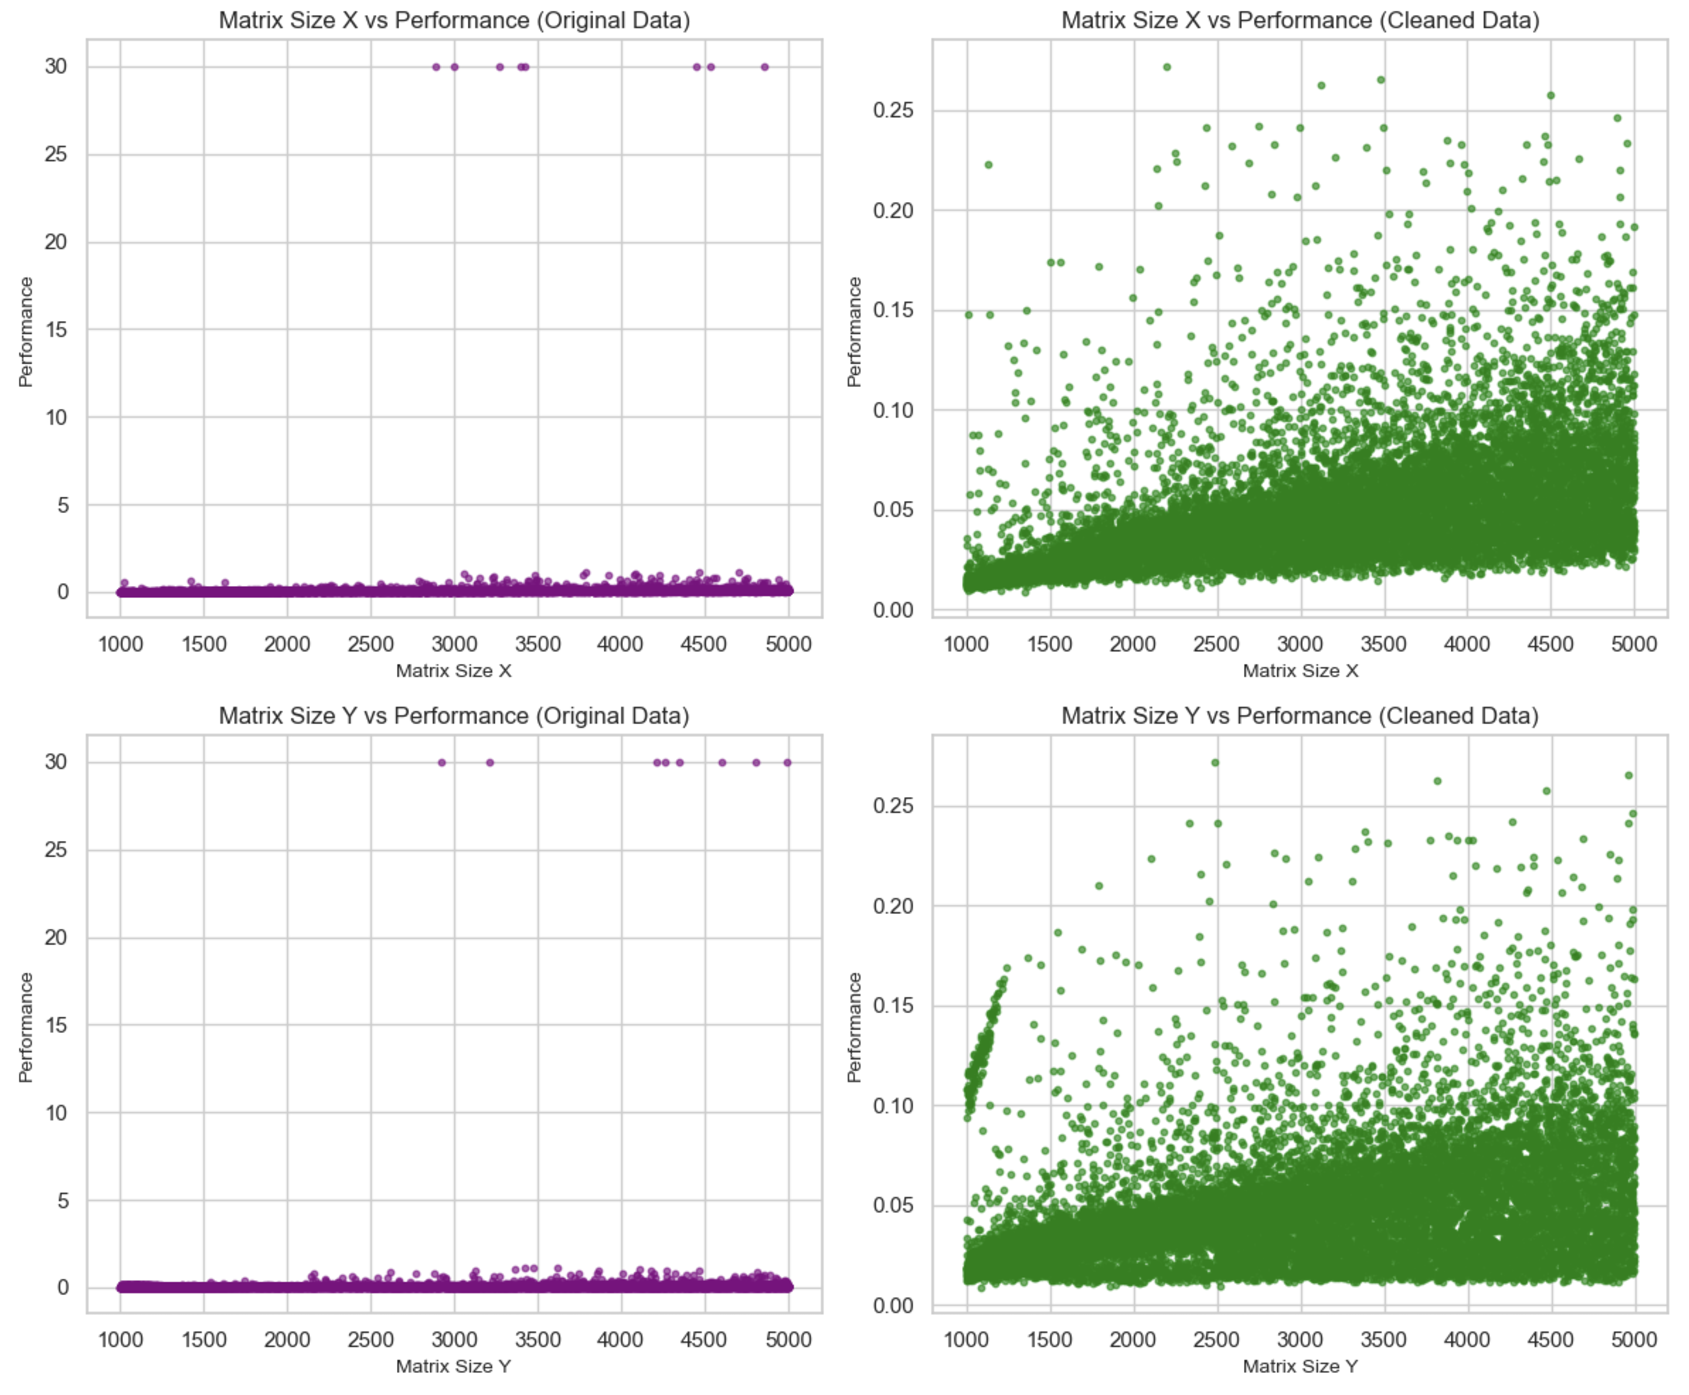
\includegraphics[width=0.6\textwidth]{logos/data_clean.jpg} 
    \caption{Comparaison de la taille de la matrice et des performances avant et après le nettoyage des données} 
    \label{fig:data_clean}
\end{figure}









\section{Méthodes ensemblistes (Ensemble learning)}

\subsection{Bagging}
Le Bagging, ou Bootstrap Aggregating, est une méthode d’ensemble utilisée pour améliorer la précision et la robustesse des modèles d’apprentissage supervisé, notamment dans le cadre des arbres de décision. L’idée principale consiste à entraîner plusieurs modèles indépendants sur des échantillons aléatoires tirés avec remise des données d’entraînement (bootstrap) et à agréger leurs prédictions pour réduire la variance et limiter les effets des données bruitées ou aberrantes. 
\subsubsection{Construction de l'ensemble de modèles}
Dans cette implémentation, la fonction \func{bootstrapSample} génère des échantillons aléatoires avec remise à partir des données d'origine. Ces échantillons, bien que de taille identique à celle du jeu de données initial, contiennent souvent des duplications, garantissant une diversité dans les ensembles utilisés pour l’entraînement. Ensuite, chaque arbre de décision est construit indépendamment sur un échantillon bootstrap grâce à la méthode \func{train}, qui utilise des arbres simples (\var{DecisionTreeSingle}) pour minimiser la variance.

\subsubsection{Agrégation des prédictions et évaluation des performances}
Une fois tous les arbres entraînés, le modèle combine leurs prédictions pour un nouvel échantillon en utilisant la méthode \func{predict}. Cette agrégation, réalisée par une moyenne dans les problèmes de régression, permet d’obtenir une estimation plus stable et robuste. Enfin, la performance globale du modèle est mesurée à l’aide de la fonction \func{evaluate}, qui calcule l’erreur quadratique moyenne (MSE) sur un ensemble de test. Cette approche garantit une prédiction plus fiable et robuste aux variations des données initiales.

\subsection{Boosting}
Le Boosting est une méthode d’ensemble qui renforce les modèles faibles, comme les arbres de décision, pour obtenir un modèle prédictif plus performant. Dans cette implémentation, la classe \var{Boosting} utilise des arbres de décision (\var{DecisionTreeSingle}) comme base et applique une méthode séquentielle pour réduire les erreurs résiduelles. Chaque arbre est entraîné à corriger les prédictions du modèle précédent, avec un contrôle exercé par un taux d’apprentissage (\var{learning_rate}) et une fonction de perte personnalisée via la classe \var{LossFunction}. Cette dernière permet de définir le comportement du Boosting en calculant les résidus et l’erreur globale.
\subsubsection{Entraînement séquentiel et correction des erreurs}
La méthode principale d'entraînement, \func{train}, commence par une initialisation avec \func{initializePrediction}, qui fixe une prédiction de départ basée sur la moyenne des valeurs cibles. À chaque itération, les résidus sont calculés en utilisant la méthode \func{negativeGradient} de la fonction de perte associée. Ces résidus, représentant les erreurs des prédictions actuelles, servent ensuite de nouvelles cibles pour entraîner un arbre de décision. La fonction train des arbres ajuste le modèle pour minimiser les résidus, et les prédictions de l’arbre sont intégrées au modèle global avec un facteur de pondération déterminé par le taux d’apprentissage. À chaque étape, la fonction de perte est réévaluée avec \func{computeLoss}, permettant de surveiller l’évolution de l’erreur.







\section{Evaluation et performance}
\lipsum[6]
\subsection{K-fold cross validation}
\subsection{Performance}

\section{Bibliographie}

\textbf{Insérer une image}
\begin{figure}[H]
    \centering
    
\includegraphics[width=0.5\textwidth]{logos/logo.png}
    \caption{Insérer une image.}
    \label{fig:logo}
\end{figure}

ou la version raccourcie avec \texttt{\textbackslash insererfigure} : \insererfigure{logos/logo.png}{0.5\textwidth}{Insérer une image avec une commande.}{logo_raccourci}


\textbf{Citer une figure} avec \texttt{\textbackslash ref} : \ref{fig:logo_raccourci}.\\


\textbf{Insérer des expressions mathématiques} en bloc :
\begin{equation*}
    \int_{-\infty}^{\infty} e^{-x^2} \, \text{d}x = \sqrt{\pi}
\end{equation*}

ou bien en \textit{inline} : $\int_{-\infty}^{\infty} e^{-x^2} \, \text{d}x = \sqrt{\pi}$.\\


\textbf{Insérer une série de calculs}
\begin{align*}
    x &= 0.999\ldots \\
    10x &= 9.999\ldots \\
    10x - x &= 9.999\ldots - 0.999\ldots \\
    9x &= 9 \\
    x &= 1 \\
    0.999\ldots &= 1
\end{align*}


\textbf{Insérer une liste}
\begin{itemize}
    \item Premier niveau
    \begin{itemize}
        \item Deuxième niveau
        \item Un autre élément au deuxième niveau
    \end{itemize}
    \item Un autre élément au premier niveau\\
\end{itemize}


\textbf{Insérer un tableau simple} \\
\begin{table}[H]
    \centering
    \begin{tabular}{|c|c|c|}
        \hline
        A & B & C \\
        \hline
        1 & 2 & 3 \\
        4 & 5 & 6 \\
        \hline
    \end{tabular}
    \caption{Un tableau simple.}
    \label{tab:tableau_simple}
\end{table}


\textbf{Insérer du code} : \texttt{print("Hello, World!")}.\\


\textbf{Insérer et référencer une boîte de code} : 
\hyperref[exemple_code]{Code \ref*{exemple_code}}.\\
Attention : le label (ici, \texttt{exemple\_code}) doit être écrit deux fois lors du référencement. Une fois dans le premier argument de \texttt{\textbackslash hyperref}, puis une seconde fois dans \texttt{\textbackslash ref*} :

\begin{center}
\texttt{\textbackslash hyperref[exemple\_code]\{Code \textbackslash ref*\{exemple\_code\}\}}.
\end{center}

\begin{codebox}[exemple_code]{Un exemple de boîte de code \texttt{Python}}
\begin{minted}{python}
def sieve_of_eratosthenes(n):
    '''Returns a list of all prime numbers up to n.'''
    primes = [True] * (n + 1)
    primes[0] = primes[1] = False  # 0 and 1 are not prime numbers
    for i in range(2, int(n**0.5) + 1):
        if primes[i]:
            for j in range(i * i, n + 1, i):
                primes[j] = False
    return [i for i, is_prime in enumerate(primes) if is_prime]
\end{minted}
\end{codebox}


\textbf{Citer une source} depuis \texttt{biblio.bib} avec \texttt{\textbackslash cite} : \cite{exemple_de_source}.\\


\textbf{Afficher une bibliographie} rapidement avec \texttt{\textbackslash insererbiblio}.

\insererbiblio 

\end{document}